\documentclass[a4paper, 12pt]{article}

\def \patha {} %Pfad zu den Dateien Preamble.tex, Commands.tex, Erwartungsbild.tex

\input{\patha/Preamble.tex}

\onehalfspacing

\newcommand{\KopfzeileBlank}{true}
\newcommand{\FACH}{Informatik}
\newcommand{\KLASSE}{5}
\newcommand{\DATUM}{XX.YY.ZZZZ}
%% Über den jeweiligen Typ wird bei Klassenarbeit und Leistungskontrolle das Erwartungsbild und der Notenspiegel als anhängende Seite kompiliert. Der Befehl \aufgabe besitzt beim Typ Arbeitsblatt einen Parameter für die Aufgabenstellung. Bei den Typen Klassenarbeit und Leistungskontrolle kommen noch zwei weitere Parameter für die Punktzahl und das Erwartungsbild hinzu.
\newcommand{\TYP}{Arbeitsblatt}
%\newcommand{\TYP}{Klassenarbeit}
%\newcommand{\TYP}{Leistungskontrolle}
\newcommand{\EINHEIT}{Bilder und Grafiken gestalten}
\newcommand{\THEMA}{Rastergrafiken gestalten}
\newcommand{\LEHRER}{Ti}
\newcommand{\TIME}{Zeit}
\newcommand{\NTA}{Hier ist Platz für Nachteilsausgleiche!}
%% Dieser "Switch" bewirkt, dass für Lückentexte die Lösung angezeigt oder ausgeblendet wird. Aktuell werden die Lücken jedoch noch nicht berücksichtigt. Vielleicht gibt es auch eine bessere Lösung für diesen "Switch"...
%\newcommand{\LOSUNG}{true}
\newcommand{\LOSUNG}{false}

%\input
\input{\patha/Commands.tex}

\Large

\begin{document}
\TITEL
\vspace{-1cm}
\begin{LKtext}

\aufgabe{}
	\begin{minipage}{0.65\textwidth}\vspace{0pt}
	\textbf{Vervollständige} den Lückentext.
	
		Das nebenstehende Bild ist \lk{acht} Raster breit und \lk{acht} Raster hoch. Die auftretenden Farben sind \lk{schwarz}\newline und \lk{schwarz}.	
	\end{minipage}
	\hfill
	\begin{minipage}{0.25\textwidth}\vspace{0pt}
		
\includegraphics[width=\linewidth]{A_1.png}
	\end{minipage}

\aufgabe{}
	\begin{minipage}{0.65\textwidth}\vspace{0pt}
		\textbf{Zeichne} eine der folgenden Figuren als \textbf{Rastergrafik}.

		\begin{itemize}
			\setlength\itemsep{-0.2em}
			\item Smiley
			\item Pferd
			\item Katze
			\item selbstgewähltes Motiv
		\end{itemize}

	\end{minipage}
	\hfill
	\begin{minipage}{0.25\textwidth}\vspace{0pt}
		
\includegraphics[width=\linewidth]{A_2.png}
	\end{minipage}

\aufgabe{}
	\begin{minipage}{0.65\textwidth}\vspace{0pt}
		\textbf{Vergleiche} den Smiley aus Aufgabe 1 mit der nebenstehenden Zahlenmatrix. Beschreibe, was die \texttt{1} und die \texttt{0} jeweils bedeuten.\newline
		Die \texttt{1} bedeutet \liniert[]{1}
		Die \texttt{0} bedeutet \liniert[]{1}
	\end{minipage}
	\hfill
	\begin{minipage}{0.25\textwidth}\vspace{0pt}
		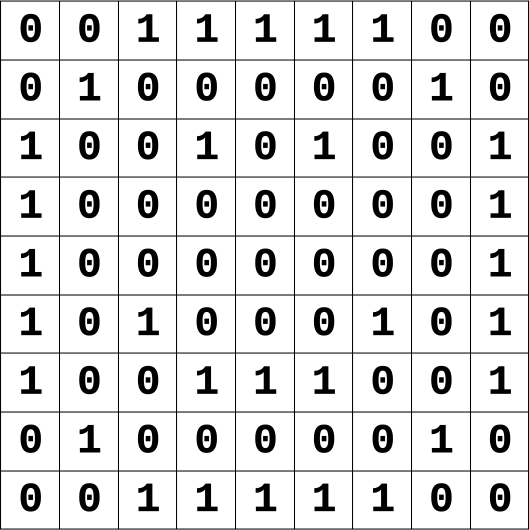
\includegraphics[width=\linewidth]{A_3.png}
	\end{minipage}
	
\aufgabe{}
	\begin{minipage}{0.65\textwidth}\vspace{0pt}
		\textbf{Erstelle}  eine Zahlenmatrix zu deinem Rastergrafik aus \textbf{Aufgabe 2}.
	\end{minipage}
	\hfill
	\begin{minipage}{0.25\textwidth}\vspace{0pt}
		
\includegraphics[width=\linewidth]{A_2.png}
	\end{minipage}

\aufgabe{}
	\textbf{Erstelle} ein Haus als Rastergrafik. Das Bild soll folgende Eigenschaften aufweisen:
	\begin{itemize}
	\setlength\itemsep{-0.2em}
		\item Der Rahmen ist \textbf{1} Rasterpunkt breit
		\item Das Haus ist genau \textbf{8} Rasterpunkte breit
		\item Das Haus ist genau \textbf{12} Rasterpunkte hoch (Bis zur Dachspitze)
		\item Das Dach des Hauses ist ein Spitzdach und ist an der untere Kante genau \textbf{10} Rasterpunkte breit
		\item Das Haus hat mindestens ein Fenster
		\item Das Haus hat eine Tür
		\item Ein Hintergrund soll vorhanden sein
	\end{itemize}
	Du kannst das Haus noch mit weiteren Elemente dekorieren. Wähle  sinnvolle Farben für dein Haus, das Dach und den Hintergrund, sodass die Details erkennbar sind.

	\textbf{Beachte:} Ein Kästchen darf nur komplett mit \textbf{einer} Farbe ausgemalt werden.
	
	\kariert[7]{7}

\end{LKtext}

\label{LastPage}
\normalsize
%\input
\ifthenelse{\equal{\TYP}{Klassenarbeit}}{
\input{\patha/Erwartungsbild.tex}}
{}
\ifthenelse{\equal{\TYP}{Leistungskontrolle}}{
\input{\patha/Erwartungsbild.tex}}
{}


\end{document}